% vim: set spelllang=fr foldmethod=marker:
\section{Simulation du processus}\label{se:sec:simul}

    \subsection{Résultats numériques}
Le processus de sélection des \cns selon leur énergie résiduelle a, lui aussi, conduit à la réalisation de plusieurs simulations, afin de le comparer au modèle de sélection pseudo-aléatoire.
Le logiciel \nsiii~\cite{ns3} a été utilisé pour l'occasion.

Plusieurs instances de simulation ont été réalisées, avec l'accent porté sur les valeurs de l'énergie consommée ainsi que sur la répartition de la charge dans le cluster.
Les mécanismes de détection des deux méthodes sont quasiment identiques, et fournissent donc des résultats similaires à ceux obtenus au chapitre précédent en \ssref{sa:ssec:detec} (sur la méthode avec renouvellement périodique) pour ce qui est du taux de détection des nœuds compromis.
Les paramètres utilisés lors des simulations sont présentés en \tabref{se:table:parameters}.

\begin{table}[!ht]
    \centering
    \caption{Paramètres de simulation}
    \medskip
    \begin{tabular}{l l}
        \toprule
        \textsc{Paramètre}                 & \textsc{Valeur}\\
        \midrule
        Nombre de nœuds                    & 30 (plus 1~\CH)\\
        Nombre de \cns                     & 4\\
        Probabilité de sélection d'un \vns & 33~\%\\
        Période de renouvellement des \cns & 1~minute\\
        Durée totale de simulation         & 30~minutes\\
        Forme du cluster                   & carré\\
        Taille du cluster                  & 2$\times$50~mètres de diagonale\\
        Portée de transmission             & 50~mètres\\
        Position des nœuds                 & \CH: au centre; autres: aléatoire\\
        Mobilité des nœuds                 & nulle\\
        Débit d'émission des nœuds normaux & 1024~octets toutes les 3~secondes\\
        Requêtes des \vns (par \cn cible)  & 1024~octets toutes les 5~secondes\\
        \bottomrule
    \end{tabular}\label{se:table:parameters}
\end{table}

Ces simulations ont permis d'obtenir l'énergie résiduelle de chaque capteur à intervalles réguliers (une fois par minute).
À partir de ces données, nous avons pu retracer les courbes d'évolution de la moyenne et de l'écart-type de la distribution de l'énergie résiduelle entre les nœuds.
L'énergie résiduelle du \ch a été volontairement ignorée.
\begin{figure}[!b]
    \centering
    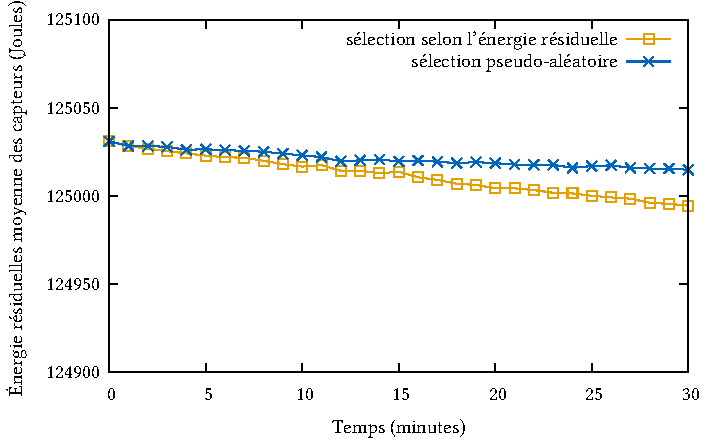
\includegraphics[width=.96\linewidth]{\chapterfig/plot_se_mean.pdf}
    \caption[Valeur moyenne de l'énergie des nœuds en fonction du temps]{Valeur moyenne de l'énergie des nœuds (à l'exception du \ch) en fonction du temps}\label{se:fig:mean}
\end{figure}
La valeur moyenne est présentée sur la \figref{se:fig:mean}.
L'augmentation des valeurs à $t=11$~minutes ainsi qu'à $t=15$~minutes sur la courbe de la sélection par l'énergie provient de l'effet de récupération des batteries.
Ces résultats sont conformes aux attentes: le processus de sélection par l'énergie consomme davantage d'énergie dans le réseau, ce que l'on peut imputer au rôle supplémentaire de \vn mis en place.
Étant donné que les \vns vont avoir à sortir périodiquement de leur état de veille pour envoyer une requête au \cn surveillé, écouter la réponse, et calculer une consommation théorique, le besoin en ressources énergétiques se retrouve logiquement affecté par rapport au processus de sélection pseudo-aléatoire.

Le volume de données de contrôle pour les deux méthodes proposées apparait sur la \figref{se:fig:overhead}.
Ici encore, l'usage des \vns entraine une augmentation des ressources consommées; il faut également tenir compte des messages (moins nombreux) envoyés par chaque capteur au moment du renouvellement de la sélection.
\begin{figure}[!ht]
    \centering
    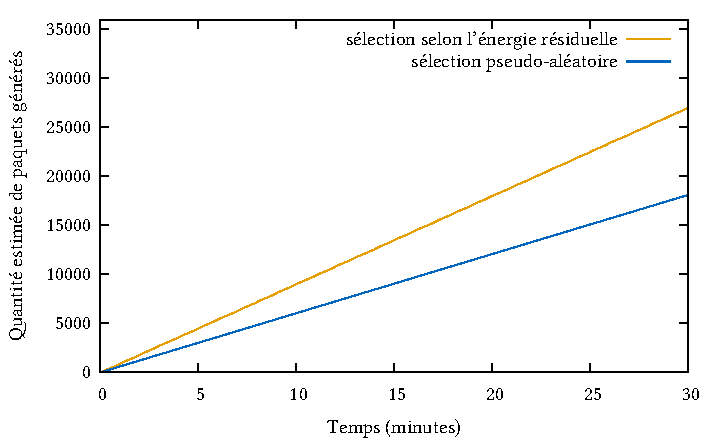
\includegraphics[width=.96\linewidth]{\chapterfig/plot_se_overhead.pdf}
    \caption{Estimation du nombre total de paquets générés au cours de la simulation au cours du temps}\label{se:fig:overhead}
\end{figure}

L'écart-type de la distribution en énergie résiduelle des nœuds est présenté sur la \figref{se:fig:stddev}.
Durant les premières minutes de la simulation, la sélection par l'énergie crée une dispersion plus affirmée de la charge en énergie du réseau, à cause des \vns (il y a davantage de capteurs qui endossent des rôles consommant plus d'énergie).
Mais après les sept premières minutes environ, l'écart-type pour le processus de sélection par l'énergie devient et demeure inférieur à celui associé à la méthode pseudo-aléatoire.
Cela traduit la meilleure répartition de la charge énergétique dans le cluster, ce qui était l'objectif initial de la solution proposée dans ce chapitre.
La différence entre les écart-types des deux méthodes est malgré tout peu élevée: cela tient entre autres aux modèles implémentés pour les simulations.
Comme nous disposons d'un générateur de nombres pseudo-aléatoires efficace, à partir d'un certain nombre de renouvellements de la sélection, tous les capteurs vont endosser le rôle de \cn à peu près le même nombre de fois si la sélection se fait de façon pseudo-aléatoire.
Et comme les capteurs ont également des activités de mesure identique, cette méthode (pseudo-aléatoire) fournit, dans notre cas, une excellente répartition de la charge dans le cluster.
Dans une situation où les capteurs auraient des niveaux d'activité différents ---~si par exemple un évènement à détecter se produit beaucoup plus souvent dans une certaine région géographique du cluster~--- alors la consommation, avec cette méthode, ne serait plus nécessairement équilibrée entre tous les nœuds du cluster.
Tandis que la sélection des \cns par l'énergie résiduelle permettrait de rétablir cet équilibre.
\begin{figure}[!ht]
    \centering
    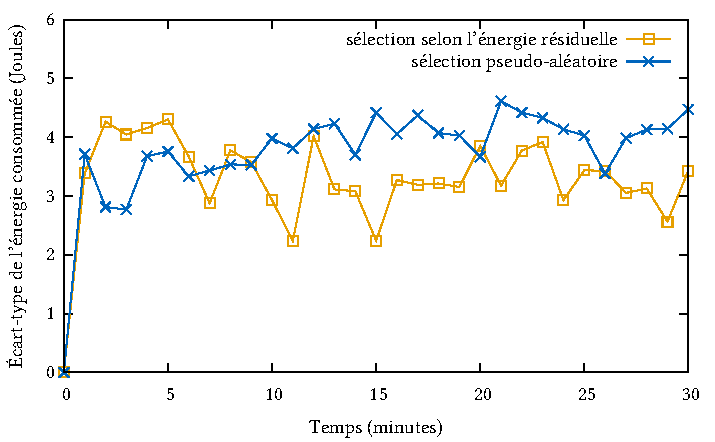
\includegraphics[width=.96\linewidth]{\chapterfig/plot_se_stddev.pdf}
    \caption[Écart-type pour l'énergie résiduelle des nœuds au cours du temps]{Écart-type pour l'énergie résiduelle des nœuds (à l'exception du \ch) au cours du temps}\label{se:fig:stddev}
\end{figure}

    \subsection{Pousser plus loin l'amélioration}

Par rapport au processus d'auto-désignation pseudo-aléatoire introduit dans le chapitre précédent, le second mécanisme proposé prend en compte l'énergie résiduelle de chaque nœud au moment de renouveler les \cns, ce qui assure une meilleure répartition de la consommation en énergie dans le cluster.
Mais si elle est mieux répartie, l'énergie consommée l'est aussi en plus grande quantité, principalement à cause de l'usage nouveau des \vns.
Les requêtes et les réponses aux \cns consomment de l'énergie, et viennent alourdir l'implémentation de la solution: il y a trois rôles différents assignés dans le cluster (sans compter le \ch), et deux d'entre eux nécessitent une étape spécifique pour leur attribution.

Il serait commode de pouvoir se passer des \vns, mais sans faire de concessions sur la sécurité.
L'idéal serait de pouvoir réutiliser les observations des \cns antérieurs pour mettre en place un mécanisme de sélection qui tienne compte de l'énergie résiduelle, voire même d'un ensemble de paramètres permettant de choisir les meilleurs candidats.
Ce jeu de paramètres, s'il inclue un score de confiance, peut même venir renforcer la sécurité du dispositif.
C'est sur cet axe que s'appuient les améliorations proposées dans le prochain chapitre.
